\chapter{Implementation}

\section{Client Implementation}
\subsection{Mapping}
The first iteration focused on the central component of the application, the map. It was vitally important that an appropriate mapping solution was used. It needed to both be functional and beautiful. As it was the main influence on the applications aesthetics the cartography needed to be pleasing on the eye. As well as looking nice it need to function as an easy to read map that let units stand out clearly from other static mapped features.

\subsubsection*{Google}
The original investigation focused on Google's own mapping solution. They provide a simple, easy to use interface to their own maps making it the obvious choice for any Android application. Their maps are accurate, up-to-date and very detailed.

Unfortunately there are a number of restrictions in place stopping their use in a number of situations. The most relevant of which is that they can not be used in an application that is not freely available to the public. Therefore restricting it's use in a paid-for application, such as MapWars may become. As the future of the application is uncertain it seemed desirable to steer clear of as many possible restrictions as possible. For this reason it was important to find a comparable alternative.

\subsubsection*{OpenStreet Map}
OpenStreet map is a publicly contributed, free world map. It's growing popularity means that the majority of developed countries are mapped to an incredibly high standard, with other countries not far behind. With an acceptable level of detail combined with it's open standards made it the next most obvious source.

OSM has an API that allows it to be easily embedded into webpages but no native android SDK. A number of 3rd party libraries are available. The most complete and popular is that provided by MapQuest.

MapQuest are a mapping company that combines proprietary data and OSM data to create their own maps. They offer an Android SDK that gives you the option of which tile source to use. There are obviously restrictions to the proprietary data but if you opt for the free tiles then the same license is used as with OSM. The Android SDK available was designed to mirror the API available for the Google Map SDK. This made swapping out the Google Maps code and replacing it with the MapQuest code was trivial and problem free.

At the point in time of implementing MapQuest the design had called for the option to switch between satellite and road maps. MapQuest's main drawback, and more widely OSM itself, was it's lack of detail. The level of zoom supported was a number of levels less than that of Google Maps. These extra zoom levels would have made unit manipulation easier on smaller devices. Satellite images were the main concern as they were not available at the level of zoom required to make game play comfortable.

MapQuest was used as the mapping solution for a large portion of development and offered a stable platform. Once more of the functionality was in place user testing presented a number of problems with the map tiles being used. Most significant of which was a difficulty in being able to locate units among the details presented with the map. The sprites and colours being used to represent units were experimented with but none were clearly visible. The problem was with the design of the tiles being used and not necessarily the zoom levels present, although this may have helped alleviate the problems.

\subsubsection*{MapBox}
One option available was to use a tile creator and host the map tiles on a server. This would be a costly and difficult solution to the problem. Hosting tiles is not a trivial task and require large amounts of storage and bandwidth.

MapBox offer beautifully customizable hosted tiles. They also have their own software called TileMill which allows the creation of bespoke tiles based on any data source which can then be hosted and distributed via their network. TileMill was based on a CSS style syntax allowing you to customise any visual aspect, from line widths, colours, strokes. It also had the ability to import data from any source giving the ability to build up rich tiles with as much detail as required. For MapWars only the most basic detail was required while using a simple colour pallet. The idea was to make any unit stand out against the map while still presenting all the information required to orientate the user with their surroundings. 

Tiles could be loaded from MapBox using a standard URI syntax used by the most tile vendors. This allowed it to integrate easily into any mapping framework.All that was needed was an SDK that allowed custom tile sources. Such functionality was found in OSMDroid\footnote{http://code.google.com/p/osmdroid/}. Like with MapQuest, OSMDroid followed the same pattern as Google Maps allowing it to be easily placed into the application without only one substantial problem. OSMDroid was missing one function that was supported by both Google Maps and MapQuest. These function was key in selecting units so had to be reimplemented ... which was not difficult but took time. Assumption was made it would be as effortless as the previous transition. After integration was complete plugging in the URI to my generated tiles was simple and worked straight of the bat.

MapBox did not offer satellite imagery but the beauty and simplicity of the maps being used made up for this. It was also decided that the complexity of such maps would just present the same images as found with the default OSM tiles. Satellite images could always be added to OSMDroid by simply finding a tile source and using that and would have no affect on the functionality of the application. 


\subsection{Location}
Detecting the users location accurately is fundamental and is used directly in controlling game play throughout the game.

There are a number of difficulties presented when trying to accurately determine a users location. Firstly is the array of different providers available, each with their own unique characteristics, advantages and disadvantages.

Getting location updates within the application code was straightforward. Android exposes location updates by subscribing to providers via the LocationManager. A LocationListener can subscribe to any number of location providers and specify the frequency of updates required. Updates are sent after a minimum time and distance is reached. For this application battery life was more of a concern than getting high precise to the second data. So the minimum time between updates was set to one minute and the minimum distance sent to 2 meters. The minimum distance did not directly save battery but eliminates noise and recalculations based on small movements.

The network location provider uses the phones network connections to try and determine the users location. If they are connected via Wi-Fi the SSID (Service Set Identifier) is queried against Google's database of known SSID's, returning a location. This database is built by crowd sourcing data from Android handsets. When enabling location services on an Android device the following messages is displayed, \"Allow Google's location service to collect anonymous location data\". Periodically the users location data from GPS, Cell-ID and Wi-Fi is broadcast along with details about available Wi-Fi connections to Google. This data tends to be fairly accurate, however when not connected to Wi-Fi the network location provider returns a location based upon Cell-ID. This technique identifies the mobile network providers cell the users is in. The location of each Cell-ID can be located so an estimated can be produced for the users location. Unfortunately cells can be very large making this method very inaccurate, however this tends to be around 1km and even less within rural locations\cite{1377314} making it acceptable for this application.

When taking location data from a variety of sources it is critical to have a process to determine which is the most accurate to the users current location. The developers guide on location strategies\cite{location} was an ideal resource to understand how each different provider worked and ultimately how to combine them to produce the best outcome. Each provider will gather data at different times and to a different level of accuracy. Whenever this data is processed a judgement needs to be made into whether this is more reliable than the currently known location. This was made based on its accuracy and age.

The process used to determine the most accurate location was adapted from an example provided in the developer guide. As shown in figure \ref{fig:location} each new location is compared against different aspects of the previously known location to decide if it is more or less accurate. If no previous location has been noted then the new data is taken to be the most accurate. If there has been a previous location the new location is only used if it is significantly newer else, if it is not significantly older, the accuracy of the two sources are compared. Each time a new location is received it comes with an estimated accuracy. This accuracy is measured in meters and is defined as the radius of 68\% confidence\cite{location_accuracy}. Meaning that there is a 68\% chance that the user is located within a circle with a radius of the accuracy, mapped around the supplied location.

\begin{figure}[H]
  \centering
   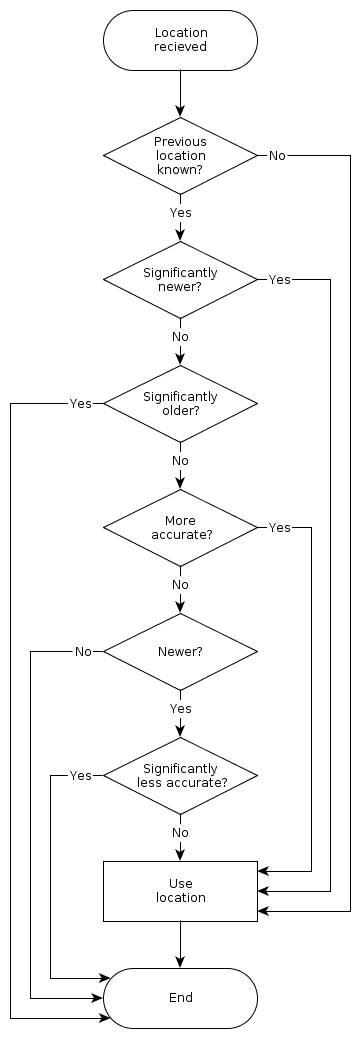
\includegraphics[height=0.9\textheight]{Images/diagrams/location.png}
  \caption{Flowchart showing the reasoning involved when selecting a location provider}
  \label{fig:location}
\end{figure}


\subsection{GUI}
\subsubsection*{Device Specific Layouts}
Android layouts offer a variety of options to provide different layouts to different devices. The most basic of which is to make a fluid layout that stretches to fill the screen using \verb|wrap_content| or \verb|match_parent| widths. As well as these options there is a variety of dimension units to allow layouts adjust to different devices. The most useful of which are density-independent pixels (dp) which are units based on the physical screen size. These units relates to one pixel on a 160 dots per inch (dpi) screen. So the ratio of dp-to-pixel changes to match a devices dp. There is also a derivative of dp, scale-independent pixels (sp). Sp is the same as dp but also takes the users font size preferences into account.

Although flexible layouts allow for a single layout to be used across devices it does not allow for different layouts to be specified. This is possible using size-specific resources\cite{screensizes}. By placing layouts in a folder \verb|layout-large| these layouts will only be used for devices classified as large, where any device below this category will use layout files in the standard \verb|layout| folder. These size qualifiers are predetermined and static As of Android 3.2 new smallest width based qualifiers were introduced using the devices dp as a reference. Layout files placed in a folder \verb|layout-sw<n>dp| are used only for devices with a minimum width of n dp. It is noted that a typical 7" tablet has a minimum width of around 600dp, this is the size opted for in this project. As described in the design it was important to differentiate between the phone and tablet layouts as both offer users a different experience.

While working on two separate layouts a large amount of code was being repeated and as features were added both layouts had to be updated interdependently. This seemed like a waste of time so a neater solution was investigated. A simple yet elegant solution was found that allowed different layouts to be combined together using the include tag.

For example the game screen added components to a basic map view, shown in figure \ref{fig:isogui}. The layers A and B are stored in separate files with two versions, one for each device. A simplified version of the file structure used can be seen in figure \ref{fig:fs}. \verb|map.xml| is the layout file used by the game activity, which in turn includes the header (A in figure \ref{fig:isogui}) and controls (B in figure \ref{fig:isogui}) layout files. These are automatically loaded from the correct folder on inclusion so the tablet layout is shown for devices with a width greater than 600dp.

\begin{figure}[H]
\dirtree{%
.1 res.
.2 layout.
.3 map\_controls.xml.
.3 map\_header.xml.
.3 map.xml.
.2 layout-sw600dp.
.3 map\_controls.xml.
.3 map\_header.xml.
}
\caption{Simplified layout file structure}
\label{fig:fs}
\end{figure}

\subsubsection*{Device Based Orientation}
From the design specifications for the GUI it was decided that devices of different screen sizes should not only have different layouts but also different orientations. Forcing an application wide orientation is straightforward. By setting \verb|android:screenOrientation| to landscape in the \verb|AndroidManifest.xml| file will keep the orientation landscape. Unfortunately there is not such a simple solution for setting the orientation based on device.

It is also possible to set the orientation within the application code. Each activities orientation can be set using \verb|Activity.setRequestedOrientation|. Once it has been determined which device is being used it is then possible to set the relevant orientation, as shown in figure \ref{fig:orientation}. It is to be noted that this changes the orientation for this activity, not the application. As the application is built of multiple activities this needs to run whenever a new activity is created. All activities have access to the MainController and call \verb|setActivity| on creation, so this seemed like the most logical point to do this.

\begin{figure}[H]
\begin{verbatim}
if (Utils.isTablet(currentContext)) {
    currentActivity.setRequestedOrientation(
            ActivityInfo.SCREEN_ORIENTATION_LANDSCAPE);
} else {
    currentActivity.setRequestedOrientation(
            ActivityInfo.SCREEN_ORIENTATION_PORTRAIT);
}
\end{verbatim}
\caption{Setting screen orientation based upon device}
\label{fig:orientation}
\end{figure}

The code behind isTablet() was based upon an online solution\cite{istablet} to differentiate between big phones and small tablets. It appears that the best approach is to calculate the screen size by dividing the pixels by the devices dpi. A diagonal screen width of 7 inches was selected as the cut off point between classifications. Anything over this felt more comfortable in landscape orientation and are mainly operated in this manor.

\subsubsection*{9-patch Images}
9-patch images are the ideal solution for designing images that are intended to scale. As this application will be run on a variety of devices they were desirable to investigate further.

\begin{wrapfigure}{r}{0.22\textwidth}
  \centering
  
\includegraphics[width=0.1\textwidth]{Images/input_green.png}
  \caption{Text input 9-patch background image}
  \label{fig:patch}
\end{wrapfigure}

These standard images contain information that can be used to define how the image should be have when scaled. Surrounding the design are four separate, pixel wide lines that indicate which sections should scale. Those located on the north and west edge mark the area that should be scaled. When the image is stretched the areas not in-line with these marks stay as they are whereas the marked out area stretches to fill in the gap. As the side of this image is uniform it makes no difference if just one pixel stretches or a large portion, so just a single pixel was used. The other marks, east and west, are there to indicate the fill area or in other words the free space within the image. In this case the area defines where the input text should be positioned as not to overlap to overlay the rounded corners and styling. Using the file extension .9.png automatically tells Android that this is a 9-patch image and it will use the guides to scale the image. 

Only one 9-patch image was used during this project and that was to keep a consistent look across devices for text fields. When styling a text field it is important to give the user feedback regarding which input is currently selected. For this a background was created with multiple drawable items, one for when the input has focus and the default. The image used for focused inputs is shown in figure \ref{fig:patch} showing a green glow around the input.

\subsection{Communication}
To start developing the communications portion of the client code a simple server was required. For this a basic echo server was created that simply received data and responded with a static response. With this in place it was possible to start experimenting with different technologies. The first big decision being between using push or pull technology.

Both push and pull are types of network communication and describe the interactions between the client and the server. Pull is the technique where each interaction is initiated by the client, the client sends the server a message and the server responds. Push on the other hand allows the free transmission of data in both directions irrespective of previous communications. Typically in a push scenario the client subscribes to a server so when new content is available the server pushes the data on to the client. In a push scenario data is received by the client as close to real-time as possible, whereas when using pull the server has to wait for the client to request data before it is transmitted.

In the fast pace of online multi-player games it is vital to update all clients with out players actions as quickly and accurately as possible. The standard approach is to have a highly coupled client-server architecture relying on push technology to keep all clients updated. However after reading a study\cite{6329833} examining the feasibility of using RESTful architecture for a massively multi-player game. RESTful architecture would take advantage of pull instead of the standard push. It was conclude that it is possible to support the kind of user and interaction loads found in popular multi-player games using REST, if caching and other techniques were utilized.

REST lends itself to scalable applications due to its stateless communication, meaning that re-authenticate is required for each request. This re-authentication enables each request to be processed by any server in the network, irrespective of any previous interactions. Creating a scalable server architecture would be a desirable goal any multi-player game as it allows the architecture to quickly adapt to influxes of users. Each request could be received by a transparent proxy that would forward the message on to one of the servers residing behind it. The server could then process this request, responding data will then relayed back through the proxy to the client. Having each request hit the proxy before being allocated to a server would help load balance the servers, distributing activity equally between servers. Adding in the possibility for the proxy to avoid overloaded machines until they finish their current requests. When using push this balancing becomes more complicated as the proxy will direct each new client to the least loaded server. As users connect and part one server may become overloaded as its connected clients continue to interact heavily while other servers sit idling. This would have to be combated by closing connections and having them re-established with a different server when one comes under too heavy a load.

Original spike work focused on implementing such a pull based system. It was found that, although the papers conclusion was achievable, the number of requests required to make the game playable was huge. Creating and tearing down connections is a costly and slow procedure. These drastically increased the battery usage, to try and combat this the number of updates were reduced. When reduced enough to make a difference to this battery usage the game play became outdated so quickly it was impossible to play an accurate game.

It was decided to instead opt to use a single persistent socket between the client and server. This connection allowed free passage of data both up and down stream without having to reconnect or re-authenticate. This improves both speed and efficiency. When data is received by the server, if appropriate, it is instantly transmitted to all relevant clients. Meaning data received by the client is always as fresh as possible, while only sending network traffic when new data is available. This form of communication was implemented using raw sockets. A thread executed every 100 milliseconds reading a buffered line of input from the socket and passing this to a handler in the main controller. The problem with this approach is that it does not entirely handle disconnects or changes in network interface. Resulting in some unexpected behaviour when the user loses connection.



\section{Server Implementation}
\subsection{Communication}
Server communication was handled by the twisted networking library which is a event-driven framework allowing for rapid implementation. Only two events were eventually used to track connected clients and receive data.

To enable the push style of communication it was important to keep an up to date list of connected clients. When a new connection is established the first command received must be an authentication request. Once a connection is authenticated a user object is created and stored in a list of connected users. After the connection is authenticated it can then start making other requests. If one of these requests affects game-play by creating, moving or attacking a unit all other units, within range, are notified. By looping through the list of connected users those in range can be isolated and their. A message is then transmitted to the connection obtained from their object.

\subsection{Geo Function}
Most of the functionality of the server requires calculations based upon coordinates and distance. These functions are not available inside Python so a class containing these methods was created. The mathematics involved in each function was aided by an detailed on-line resource\cite{geo} explaining how to perform different calculations on a sphere. Output from the resulting class was far from accurate as it took a simplistic view of the earth as a perfect, smooth sphere of a fix radius. It was deemed accurate enough for the required purpose.

A serious amount of time was wasted by unexpected output when requesting a bounding box around a coordinate. This was due to inexperience with the language rather than any errors in the theory. The function relied on radius been calculated by dividing the desired radius by the radius of the earth. This simple division was the root of the issue. As both values being divided were supplied as integers the returned value was also an integer. Due to the expected result being very small and precise instead of resulting in 0.0000123, for example, 0 was the given result. This 0 was then used to calculate the size of the bounding box meaning it was non existent. By adding a decimal to one of the values being used it changed it from an integer to a float thus returning a float of the correct value. Once this had been added the function worked exactly as anticipated.


\subsection{Unit Control}
Unit locations and other details are stored and queried directly in the SQLite database. As well as simply storing and transmitting unit locations the server also handles the movement of units between way points and confrontations between units.

Unit movement is handled by a fairly simple formula that took longer than expected to reach. The final algorithm was based upon Bresenham's line algorithm\footnote{http://en.wikipedia.org/wiki/Bresenham's\_line\_algorithm}, one of the simplest solutions but results in fair accuracy and minimal computation. By combing the algorithm with a calculated number of steps it was possible to visualize unit movement between two points at a consistent speed. This was achieved by basing the number of steps on the distance remaining so that as the distance decreases so does the number of steps remaining to take before the unit has reached its destination.

After all units have been relocated each unit looks for enemy units within range of its weaponry. Selecting the closest unit and removing health from it. This had the intended result but led to rigid, predictable and uninspiring behaviour. To make the combat more interesting the order in which units attacked was randomized as well as adding a probability to whether the units attack would be successful. Combined with limitations placed upon fire rates of each unit created a more dynamic experience. An uncomplicated but essential bit of reasoning that improved game-play drastically.